\subsection{Por qué la posición sola no alcanza como estado}

Como señala la guía: dos situaciones $s_1 = (5,4)$ y $s_2 = (5,4)$ pueden corresponder a la misma
posición de Pac-Man pero, si en $s_1$ ya visitó una esquina y en $s_2$ ya visitó tres, no son
estados equivalentes para este problema --requieren seguir caminos distintos para llegar a la
meta--. Por lo tanto el estado tiene que incluir, además de la posición, qué esquinas ya se
visitaron.

\subsection{Estado elegido}

$$s = (\text{posición}, \text{esquinas\_visitadas})$$

donde \texttt{esquinas\_visitadas} es una tupla de 4 booleanos, uno por cada esquina de
\texttt{self.corners} (en el mismo orden: \texttt{(1,1)}, \texttt{(1,top)}, \texttt{(right,1)},
\texttt{(right,top)}). Se eligió una tupla --no una lista-- porque el estado tiene que ser
\emph{hasheable y comparable} para funcionar dentro de \texttt{util.PriorityQueue} y de cualquier
diccionario de costos: las tuplas de booleanos cumplen ambas propiedades sin ningún esfuerzo extra
(a diferencia del \texttt{foodGrid} de \texttt{FoodSearchProblem}, que sí necesitó el contador de
desempate documentado en la Actividad 3 precisamente porque no es comparable).

\begin{figure}[H]
\centering
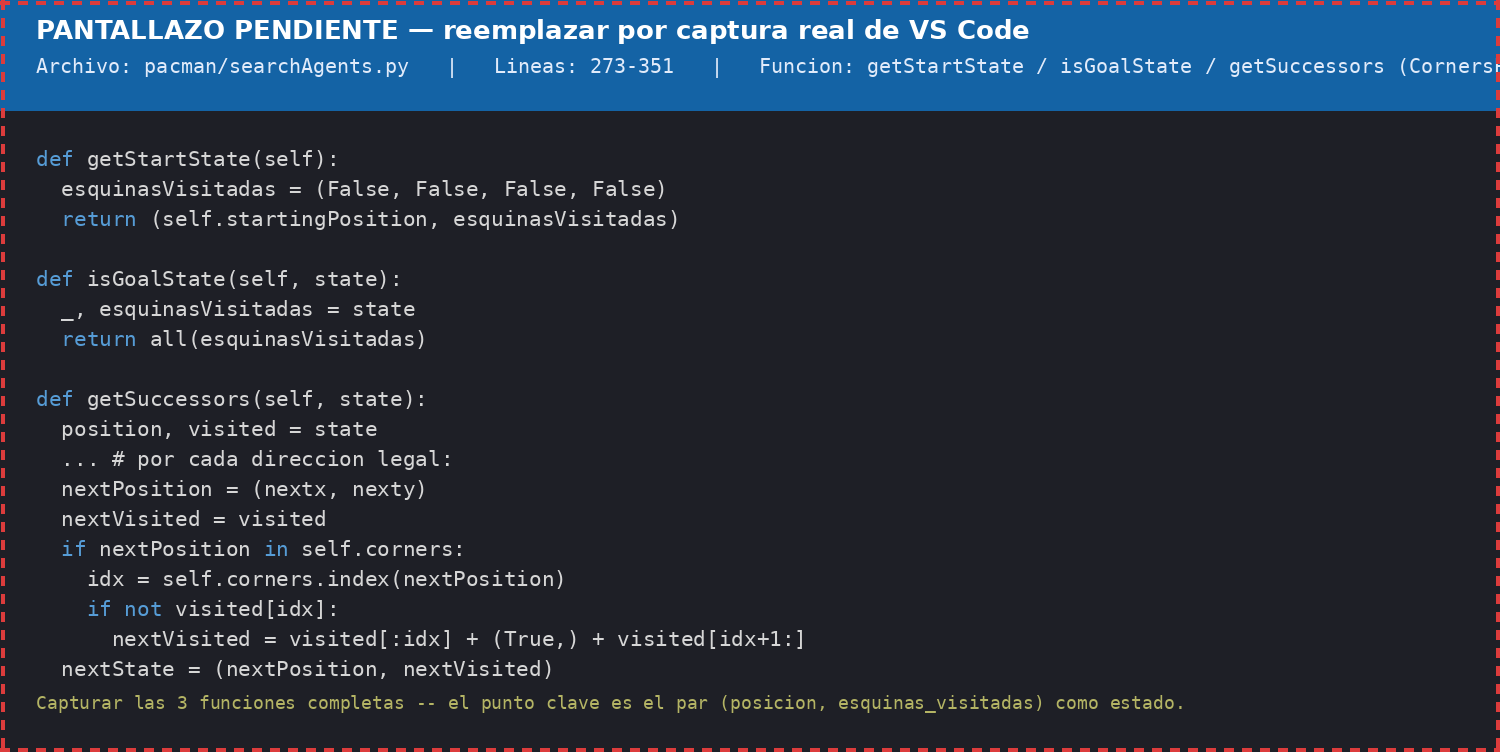
\includegraphics[width=0.95\textwidth]{capturas/actividad07_corners.png}
\caption{\texttt{getStartState}, \texttt{isGoalState} y \texttt{getSuccessors} de
\texttt{CornersProblem} en \texttt{pacman/searchAgents.py} (líneas 273-351).}
\label{fig:act07-corners}
\end{figure}

La meta se alcanza cuando \texttt{all(esquinas\_visitadas)} es verdadero --las 4 esquinas ya se
visitaron--, sin importar en qué posición esté Pac-Man en ese momento. Cada sucesor recalcula la
tupla completa de esquinas visitadas (las tuplas son inmutables, así que no se modifica
\texttt{visited} en el lugar): si la nueva posición coincide con una esquina que todavía no estaba
marcada, se genera una tupla nueva con esa esquina en \texttt{True}.

\subsection{Procedimiento y resultados}

Se ejecutó UCS sobre \texttt{tinyCorners} (ver \texttt{experimentos/actividad7\_corners\_estado.py}).

\begin{table}[H]
\centering
\caption{UCS sobre CornersProblem}
\label{tab:act7-ucs}
\begin{tabular}{lrrrr}
\toprule
\textbf{Layout} & \textbf{Costo} & \textbf{Longitud} & \textbf{Nodos expandidos} & \textbf{Tiempo (s)} \\
\midrule
tinyCorners & 22 & 22 & 295 & 0.001300 \\
\bottomrule
\end{tabular}
\end{table}

Se verificó, simulando paso a paso las 22 acciones devueltas, que el estado final es
\texttt{((1,5), (True, True, True, True))}: la solución realmente visita las 4 esquinas, no solo
pasa la prueba \texttt{isGoalState} por casualidad.

\subsection{Hallazgo: \texttt{mediumCorners} no es utilizable en esta copia del proyecto}

Al intentar usar \texttt{mediumCorners} como segundo layout de referencia (para tener un caso más
grande que \texttt{tinyCorners}), UCS terminó devolviendo una lista de acciones vacía después de
explorar apenas 36 nodos --sin haber visitado ninguna esquina--. Se investigó imprimiendo
directamente la cuadrícula de paredes (\texttt{state.getWalls()}) y se confirmó que el punto de
partida de Pac-Man en este layout queda encerrado en un cuarto de $9\times4$ celdas completamente
sellado por paredes en los cuatro lados, sin ninguna puerta de salida.

Para descartar que fuera un error de nuestra implementación de \texttt{CornersProblem}, se probó lo
mismo con \texttt{PositionSearchProblem} (código ya implementado por el profesor, sin modificar),
pidiendo un camino desde el inicio hasta la esquina \texttt{(1,1)}: UCS también devuelve una lista
vacía, confirmando que ninguna búsqueda --sin importar el problema o el algoritmo-- puede escapar
de ese cuarto en este layout. Por eso, igual que se descartó \texttt{bigMaze} en las primeras
actividades, \texttt{mediumCorners} no se usa como layout de referencia en esta entrega;
\texttt{tinyCorners} es el layout principal para las Actividades 7-9.

\subsection{Pregunta de análisis}

\textbf{¿Por qué el estado de \texttt{CornersProblem} necesita almacenar más información que
únicamente la posición \texttt{(x, y)}?}

Porque la prueba de objetivo de este problema no depende solo de dónde está Pac-Man, sino de
\emph{qué ha hecho} para llegar ahí --específicamente, cuáles de las 4 esquinas ya visitó--. Si el
estado fuera solo la posición, dos caminos que pasan por la misma celda pero con distinto progreso
(unas esquinas visitadas y otras no) se confundirían en un solo estado, y el algoritmo de búsqueda
podría marcar como `ya explorado' un estado que en realidad todavía necesita explorarse con otra
combinación de esquinas pendientes, perdiendo la garantía de encontrar la solución óptima --o
incluso de encontrar alguna solución--. Codificar el progreso (esquinas visitadas) dentro del
estado es lo que hace que dos situaciones con la misma posición pero distinto progreso sean,
correctamente, dos estados distintos.
